\documentclass[10pt,a4paper]{article}
\usepackage[top=1.4cm, bottom=1.4cm, left=1.6cm, right=1.6cm, headheight=14pt, footskip=18pt]{geometry}
\usepackage[utf8]{inputenc}
\usepackage{amsmath,amsfonts,amssymb}
\usepackage{graphicx}
\usepackage{tikz}
\usepackage{circuitikz}
\usetikzlibrary{calc,patterns}
\usepackage[most]{tcolorbox}
\usepackage{enumitem}
\usepackage{fancyhdr}
\usepackage{booktabs}
\usepackage{tabularx}
\usepackage{colortbl}
\usepackage{hyperref}

% --- Palet Warna Resmi UNIB ---
\definecolor{unibblue}{RGB}{0, 32, 96}
\definecolor{unibgold}{RGB}{197, 160, 89}
\definecolor{unibgreen}{RGB}{34, 112, 60}
\definecolor{boxbg}{RGB}{248, 250, 253}
\definecolor{linegray}{RGB}{210, 215, 225}

% --- Pengaturan Header & Footer ---
\pagestyle{fancy}
\fancyhf{}
\lhead{\footnotesize\textbf{\color{unibblue}Universitas Bengkulu} \textbar\ Program Studi S1 Teknik Elektro}
\rhead{\footnotesize\color{gray}Persamaan Diferensial (Genap 2026)}
\lfoot{\footnotesize\color{gray}Problem Set OBE \textbar\ \textbf{Video}: \url{https://youtu.be/RxoN7UaK3OI} \textbar\ \href{https://www.youtube.com/playlist?list=PLS5oOZWXZeTw}{\color{unibblue}\textbf{Playlist}}}
\cfoot{\footnotesize\color{gray}Hal. \thepage\ dari 2}
\rfoot{\footnotesize\color{unibblue}\textbf{Minggu 11: Transformasi Fourier Kontinu \& S...}}
\renewcommand{\headrulewidth}{0.6pt}
\renewcommand{\footrulewidth}{0.4pt}

\begin{document}

% ==================== HALAMAN 1 ====================
\noindent\begin{minipage}[c]{0.68\textwidth}%
  {\large\textbf{\color{unibblue}PROBLEM SET (TUGAS MANDIRI TERSTRUKTUR)}}\\[1mm]
  {\normalsize\textbf{Mata Kuliah: Persamaan Diferensial (2 SKS)}}\\[0.5mm]
  {\small\textbf{Topik Minggu 11:} Transformasi Fourier Kontinu \& Spektrum Sinyal Transien}%
\end{minipage}%
\hfill%
\begin{minipage}[c]{0.30\textwidth}%
  \begin{tcolorbox}[colback=unibblue!5,colframe=unibblue,boxrule=0.6pt,arc=2pt,left=4pt,right=4pt,top=2pt,bottom=2pt]
    \scriptsize
    \textbf{Nama:} \dotfill\\[1.2mm]
    \textbf{NPM:} \dotfill\\[1.2mm]
    \textbf{Kelas/Klp:} \dotfill\\[1.2mm]
    \textbf{Nilai Final:} \hfill \textbf{/ 100}
  \end{tcolorbox}%
\end{minipage}\par

\vspace{1.5mm}

% Kotak Sub-CPMK & Pedoman Tugas Terstruktur
\begin{tcolorbox}[colback=boxbg,colframe=unibgold!90!black,boxrule=0.6pt,arc=2pt,left=5pt,right=5pt,top=3pt,bottom=3pt,title=\textbf{\scriptsize Capaian Pembelajaran (Sub-CPMK 5) \& Pedoman Pengerjaan Tugas}]
  \scriptsize
  \textbf{Sub-CPMK 5:} Mahasiswa mampu mentransformasikan sinyal non-periodik ke domain frekuensi kontinu menggunakan Transformasi Fourier serta menganalisis respons frekuensi filter listrik.\\
  \textbf{Video Perkuliahan (YouTube):} \url{https://youtu.be/RxoN7UaK3OI} \hfill \textbf{Playlist:} \href{https://www.youtube.com/playlist?list=PLS5oOZWXZeTw}{\color{unibblue}\textbf{bit.ly/pd-unib-playlist}}\\\textbf{Ketentuan Tugas:} Kerjakan secara mandiri pada kertas folio/A4 bergaris atau laporan digital rapi. Lampirkan penurunan rumus analitis lengkap dan cetak visualisasi kode program Julia (Soal C6). Kumpulkan pada awal perkuliahan minggu berikutnya.
\end{tcolorbox}

\vspace{1.5mm}

\noindent{\textbf{\color{unibblue}\large BAGIAN I: FONDASI KONSEPTUAL \& PENURUNAN MATEMATIS}}\par
\vspace{1mm}

% Soal C1
\noindent\textbf{1. (C1 - Mengingat \textbar\ Bobot: 10 Poin)}\par\vspace{0.8mm}
{\footnotesize Tuliskan pasangan integral Transformasi Fourier kontinu $F(\omega) = \mathcal{F}\{f(t)\}$ dan Invers Transformasi Fourier $f(t) = \mathcal{F}^{-1}\{F(\omega)\}$, serta sebutkan syarat cukup Dirichlet agar suatu fungsi waktu dapat ditransformasikan ke domain Fourier.}\par

\vspace{2.5mm}

% Soal C2
\noindent\textbf{2. (C2 - Memahami \textbar\ Bobot: 15 Poin)}\par\vspace{0.8mm}
{\footnotesize Jelaskan perbedaan konseptual mendasar antara Deret Fourier (sinyal periodik, spektrum diskrit harmonisa) dengan Transformasi Fourier (sinyal aperiodik/transien tunggal, spektrum kontinu kerapatan spektral).}\par

\vspace{2.5mm}

% Soal C3
\noindent\textbf{3. (C3 - Menerapkan \textbar\ Bobot: 20 Poin)}\par\vspace{0.8mm}
\noindent\begin{minipage}[t]{0.60\textwidth}%
  {\footnotesize Sebuah sinyal pulsa eksponensial transien tunggal pemutus daya dinyatakan oleh $f(t) = V_0 e^{-a t} u(t)$ dengan konstanta redaman $a > 0$. Hitung spektrum kerapatan frekuensi kontinu $F(\omega) = \mathcal{F}\{f(t)\}$, lalu tentukan magnitudo spektrum $|F(\omega)|$ dan sudut fasa $\angle F(\omega)$ secara analitis.}%
\end{minipage}%
\hfill%
\begin{minipage}[t]{0.37\textwidth}%
  \centering
  \resizebox{0.95\linewidth}{!}{%
  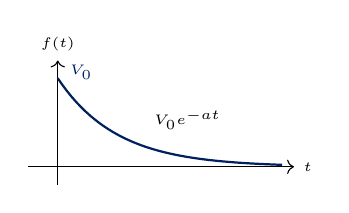
\begin{tikzpicture}[scale=0.75]
    \draw[->] (-0.5,0) -- (4.0,0) node[right, font=\tiny] {$t$};
    \draw[->] (0,-0.3) -- (0,1.8) node[above, font=\tiny] {$f(t)$};
    \draw[thick, unibblue, domain=0:3.8, samples=50] plot (\x, {1.5*exp(-1.0*\x)});
    \node at (0.4,1.6) [font=\tiny\bfseries, unibblue] {$V_0$};
    \node at (2.2,0.8) [font=\tiny] {$V_0 e^{-at}$};
  \end{tikzpicture}%
  }%
\end{minipage}\par

\vfill

% Kotak Formula Rujukan Teknis & Standar Industri
\begin{tcolorbox}[colback=unibblue!3,colframe=unibblue,colbacktitle=unibblue,coltitle=white,boxrule=0.6pt,arc=2pt,left=6pt,right=6pt,top=3pt,bottom=3pt,title=\textbf{\scriptsize FORMULA RUJUKAN TEKNIS \& STANDAR INDUSTRI TERKAIT}]
  \scriptsize
  \begin{itemize}[leftmargin=*, nosep]
  \item Pasangan Transformasi Fourier Kontinu: $F(\omega) = \int_{-\infty}^\infty f(t) e^{-j\omega t} dt$ \quad\textbar\quad $f(t) = \frac{1}{2\pi}\int_{-\infty}^\infty F(\omega) e^{j\omega t} d\omega$
  \item Teorema Modulasi Frekuensi: $\mathcal{F}\{f(t)\cos(\omega_c t)\} = \frac{1}{2}\left[F(\omega - \omega_c) + F(\omega + \omega_c)\right]$
  \item Teorema Energi Rayleigh-Parseval: $\int_{-\infty}^\infty |f(t)|^2 dt = \frac{1}{2\pi}\int_{-\infty}^\infty |F(\omega)|^2 d\omega$
  \item Respons Frekuensi Filter Pasif RC: $H(j\omega) = \frac{V_{\text{out}}(j\omega)}{V_{\text{in}}(j\omega)} = \frac{1}{1 + j\omega R C}$
\end{itemize}
\end{tcolorbox}

\newpage
% ==================== HALAMAN 2 ====================

\noindent{\textbf{\color{unibblue}\large BAGIAN II: ANALISIS SISTEM, EVALUASI STANDAR, \& KOMPUTASI JULIA}}\par
\vspace{1mm}

% Soal C4
\noindent\textbf{4. (C4 - Menganalisis \textbar\ Bobot: 20 Poin)}\par\vspace{0.8mm}
{\footnotesize Tinjau Teorema Energi Rayleigh-Parseval untuk sinyal transien: $\int_{-\infty}^\infty |f(t)|^2 dt = \frac{1}{2\pi} \int_{-\infty}^\infty |F(\omega)|^2 d\omega$. (a) Buktikan teorema ini untuk sinyal pulsa eksponensial Soal 3; (b) Tentukan bandwidth frekuensi $\omega_B$ yang memuat tepat $90\%$ dari total energi sinyal transien tersebut.}\par

\vspace{3.5mm}

% Soal C5
\noindent\textbf{5. (C5 - Mengevaluasi \textbar\ Bobot: 20 Poin)}\par\vspace{0.8mm}
{\footnotesize Sinyal transien Soal 3 dilewatkan ke filter lolos-rendah (LPF) RC satu tingkat dengan fungsi alih $H(j\omega) = \frac{1}{1 + j\omega/\omega_c}$. Evaluasi energi spektral keluaran filter $E_{\text{out}}$ dan analisis bagaimana pemilihan frekuensi cut-off $\omega_c$ meredam komponen transien frekuensi tinggi yang merusak peralatan.}\par

\vspace{3.5mm}

% Soal C6
\noindent\textbf{6. (C6 - Merancang \& Komputasi Julia \textbar\ Bobot: 15 Poin)}\par\vspace{0.8mm}
{\footnotesize Rancang skrip program dalam bahasa \textbf{Julia} menggunakan paket \texttt{FFTW.jl} untuk menghitung Fast Fourier Transform (FFT) dari pulsa persegi transien berdurasi $T = 2\text{ ms}$. Program harus memplot spektrum kerapatan energi kontinu analitis (fungsi Sinc) berdampingan dengan hasil estimasi numerik FFT.}\par

\vfill

% Tabel Rekapitulasi Skor OBE & Lembar Catatan Umpan Balik Dosen
\noindent\begin{minipage}[b]{0.62\textwidth}%
  \centering
  \scriptsize
  \begin{tabular}{|c|c|c|c|c|c|c|}
    \hline
    \rowcolor{unibblue}
    \textbf{\color{white}C1} & \textbf{\color{white}C2} & \textbf{\color{white}C3} & \textbf{\color{white}C4} & \textbf{\color{white}C5} & \textbf{\color{white}C6} & \textbf{\color{white}Total} \\
    \rowcolor{unibblue!10}
    10 Pts & 15 Pts & 20 Pts & 20 Pts & 20 Pts & 15 Pts & 100 Pts \\
    \hline
    & & & & & & \\[3mm]
    \hline
  \end{tabular}%
\end{minipage}%
\hfill%
\begin{minipage}[b]{0.35\textwidth}%
  \centering
  \scriptsize
  \textbf{Verifikasi Dosen / Asisten:}\\[6mm]
  (\dotfill)\\[1mm]
  \tiny Tanggal: \dotfill
\end{minipage}\par

\vspace{2mm}
\begin{tcolorbox}[colback=white,colframe=unibblue!40!black,colbacktitle=unibblue!10,coltitle=unibblue,boxrule=0.5pt,arc=2pt,left=5pt,right=5pt,top=3pt,bottom=3pt,title=\textbf{\tiny Catatan Evaluasi \& Umpan Balik Dosen Pengampu}]
  \tiny
  \textbf{Rubrik Pemeriksaan Pengerjaan Tugas Mandiri:}\par\vspace{0.8mm}
  $\square$ Penurunan matematis langkah-demi-langkah runtut (C1--C4) \hfill $\square$ Validasi analitis \& standar industri IEEE/IEC/SPLN akurat (C5)\\[0.8mm]
  $\square$ Skrip program Julia mandiri \& grafik visualisasi terlampir (C6) \hfill $\square$ Kerapian format laporan \& ketepatan waktu pengumpulan\\[2.0mm]
  \textbf{Catatan / Koreksi Khusus Dosen:}\\[1.6cm]
\end{tcolorbox}

\end{document}
